\chapter{Annexe technique sur les drones}
\label{chap:annexe1}

\section{Système de drone : Paparazzi}

Un drone est composé de plusieurs pièces assemblées entre elles pour former la structure sur laquelle sont fixés des actionneurs, un autopilote et une charge utile (colis, caméra, capteur, etc.). L'élément central est l'autopilote qui assure la communication entre tous les éléments. Nous pouvons décomposer l'autopilote en deux parties : la partie matérielle et la partie logicielle.
\nomenclature[]{\(PCB\)}{Circuit imprimé  \textit{Printed Circuit Board}}
La partie matérielle est constituée d'un circuit imprimé (PCB) sur lequel des composants sont installés pour assurer les tâches relatives au vol. La partie logicielle se décompose en deux éléments : le segment sol et le logiciel embarqué \ref{sec:logiciel}.

Nous pouvons détailler les capteurs embarqués et le microcontrôleur avec l'ensemble de ses ports de communication \ref{sec:capteurs} et \ref{sec:micoctrl}. 

 \subsection{Les capteurs d'un autopilote}
 \label{sec:capteurs}
 Un autopilote comporte généralement un accéléromètre, un gyroscope, un magnétomètre et un baromètre.
 
 \paragraph*{}
 \textbf{L'accéléromètre} à trois axes permet de mesurer l'ensemble des forces appliquées sur le véhicule, à l'exception du poids. Il est possible d'obtenir la position du drone par double intégration de la mesure de l'accéléromètre. Toutefois, il convient de souligner que la position dérive rapidement en raison des bruits de mesure.

 \paragraph*{}
 \textbf{Le gyroscope} à trois axes permet de mesurer les vitesses de rotation du véhicule. Il est possible d'obtenir l'orientation du drone par intégration de la mesure du gyroscope. Toutefois, comme précédemment, l'orientation dérive rapidement en raison des bruits de mesure.

 \paragraph*{}
 \textbf{Le magnétomètre} à trois axes indique la direction du nord magnétique. Il permet de se diriger par rapport à une référence connue. Le principal inconvénient de ce capteur est sa perturbation par les masses magnétiques environnantes, ainsi que par les champs magnétiques parasites induits par la proximité des moteurs électriques par exemple. Il est donc difficile de les utiliser à l'intérieur d'un bâtiment. L'influence magnétique de l'engin porteur et les perturbations dues à d'éventuels moteurs électriques peuvent être éliminées en qualifiant, de manière statique, les erreurs dues aux masses métalliques du véhicule et aux moteurs électriques (en fonction des tensions et courants d'alimentation).

 \paragraph*{}
 { \color{red}
 \textbf{Le baromètre} est un capteur d'altitude basée sur la mesure de la pression atmosphérique. Cette pression est mesure par un système électronique basée sur la résonance naturelle d'une pièce en alliage de nickel ou sur la modification de l'équilibre d'un pont de Wheatstone associé à un cristal de quartz sur lequel, par l'intermédiaire d'une capsule souple, s'exerce la pression atmosphérique. On déduit de la variation de pression atmosphérique une variation d'altitude à l'aide du modèle d'atmosphère standard qui nous indique qu'au niveau de la mer, la pression diminue de \SI{1}{\hecto\pascal} tous les \SI{8.5}{\meter}
 }

 \paragraph*{}
 \textbf{Le GPS} est monté en extérieur de l'autopilote. Ce système de géopositionnement par satellite (\textit{ Global Positioning System}) \nomenclature[]{\(GPS\)}{Géo-positionnement par satellite (\textit{Global Positioning System})} permet d'obtenir un positionnement absolu du drone. 


 \paragraph*{}
 Il est courant de retrouver plusieurs capteurs dans un même boitier, que l'on nomme centrale inertielle (Inertial Measurement Units, IMU), \nomenclature[]{\(IMU\)}{Centrales inertielles (\textit{Inertial Measurement Units})}. Ces dernières sont composées au minimum d'un accéléromètre 3-axes et d'un gyroscope 3-axes, mais il est courant de les trouver avec un magnétomètre 3-axes. 

 \subsection{Le microcontrôleur d'un autopilote}
 \label{sec:micoctrl}
 Le microcontrôleur (Microcontroller Unit, MCU) \nomenclature[]{\(MCU\)}{Microcontrôleurs (\textit{Microcontroller Unit})} est la pièce maitresse de l'autopilote en ce qu'il permet d'effectuer l'ensemble des traitements nécessaires à la conduite du vol.

 De plus il possède plusieurs ports de communication pour récupérer les données des capteurs ou envoyer des ordres aux actionneurs.


 
{\color{red}
La liaison série permet de relier deux équipements numériques pour qu'ils puissent s'échanger des informations. C'est le moyen de communication le plus simple. Toutefois, il contient de moyen de détection des erreurs tel que le bit de parité.

 Le protocole \textit{CAN} qui provient de l'industrie automobile. Il permet de raccorder à un même câble un grand nombre de calculateurs qui communiqueront donc à tour de rôle. Cette technique élimine le besoin de câbler des lignes dédiées pour chaque information à faire transiter (connexion point-à-point).

 Nous pouvons citer le \textit{Dshot} qui est un protocole de communication défini entre l'autopilote et l'ESC pour envoyer les commandes des moteurs. Les avancées sur ce protocole ont notamment permis la communication bidirectionnelle, permettant d'obtenir la vitesse des moteurs, leur consommation et d'autres informations.

 Enfin, le protocole \textit{I2C} est un bus de communication série simplifiant l'interconnexion de circuit intégré sur une même carte. Ce bus ne nécessite que deux fils pour être mis en place. Il n'est conçu que pour faire communiquer des équipements relativement proches (quelques centimètres).
}
 \subsection{Évolutions}
 Les nombreux progrès dans les systèmes d'estimation état permettent de connaître précisément l'orientation et la position des drones pour assurer la stabilisation, le guidage et la navigation. Les progrès sont liés à l'amélioration continue des capteurs, notamment des centrales inertielles constituées d'un accéléromètre, d'un gyroscope et d'un magnétomètre.

La Table \ref{tab:autopilote_ev} montre l'évolution des vitesses des microcontrôleurs (Microcontroller Unit, MCU) \nomenclature[]{\(MCU\)}{Microcontrôleurs (\textit{Microcontroller Unit})} embarqués sur les autopilotes et de la réduction du bruit des capteurs inertiels.
\begin{table}[ht]
    \centering
    \begin{tabular}{|c|c|c|c|c|c|}
        \hline
        Type & Date & MCU & Vitesse & Capteur  & Bruit RMS \\
        \hline \hline
        \href{https://wiki.paparazziuav.org/wiki/Apogee/v1.00}{Apogee}  & 2013 & STM32F4 & 168 MHz & MPU-9150 & \begin{tabular}{ccc} Gyro : 0.06 dps \\
        Accel: 4 mg  \end{tabular}  \\
        \hline
        \href{https://wiki.paparazziuav.org/wiki/Chimera/v1.00}{Chimera} & 2016 & STM32F7 & 216 MHz &  MPU-9250 & \begin{tabular}{ccc} Gyro : 0.1  dps \\
        Accel: 8 mg  \end{tabular}\\
        \hline
        \href{https://wiki.paparazziuav.org/wiki/Tawaki/v1.10}{Tawaki 1} &2019 &  STM32F7 & 216 MHz  & ICM-20600 & \begin{tabular}{ccc} Gyro : 0.04 dps \\
        Accel: 1 mg  \end{tabular}\\
        \hline
        \href{https://wiki.paparazziuav.org/wiki/Tawaki/v2.01}{Tawaki 2} &2023 &  STM32H7 & 480 MHz & ICM-42688-P & \begin{tabular}{ccc} Gyro : 0.028 dps \\
        Accel: 0.70 mg  \end{tabular} \\
        \hline
    \end{tabular}
    \caption{Évolution des autopilotes Paparazzi sur dix ans.}
    \label{tab:autopilote_ev}
\end{table}

Sur une période de dix ans, nous pouvons observer que les microcontrôleurs ont doublé leur vitesse d'exécution, que les fabricants ont divisé par deux le bruit moyen sur les gyroscopes et par quatre le bruit moyen des accéléromètres.
Ces évolutions continues permettent une amélioration de l'estimation du drone utilisée pour la stabilisation. Il en résulte une stabilité accrue et de nouvelles possibilités pour la commande des drones.

 \subsection{Les logiciels d'un autopilote}
 \label{sec:logiciel}
 Tout le fonctionnement d'un drone repose sur le logiciel qui permet de le faire voler. Il se décompose en deux catégories : la partie sol et la partie embarquée.

 \subsection{Le segment sol}
 {\color{red}
Le segment sol est un ensemble de logiciel permettant de monitorer l'état du drone et de lui envoyé des ordres. Il repose sur les informations échangées avec le drone au travers de la télémétrie. L'interface principale est la GCS \textit{Ground Control Station} (voir figure \ref{fig:GCS}), cette station de contrôle au sol assure la Visualisation du drone sur la carte, ainsi que toutes les commandes nécessaires au vol (modification de point de passage, atterrissage, etc.). Elle est écrite en C++.

\begin{figure}[ht!]
    \centerline{
    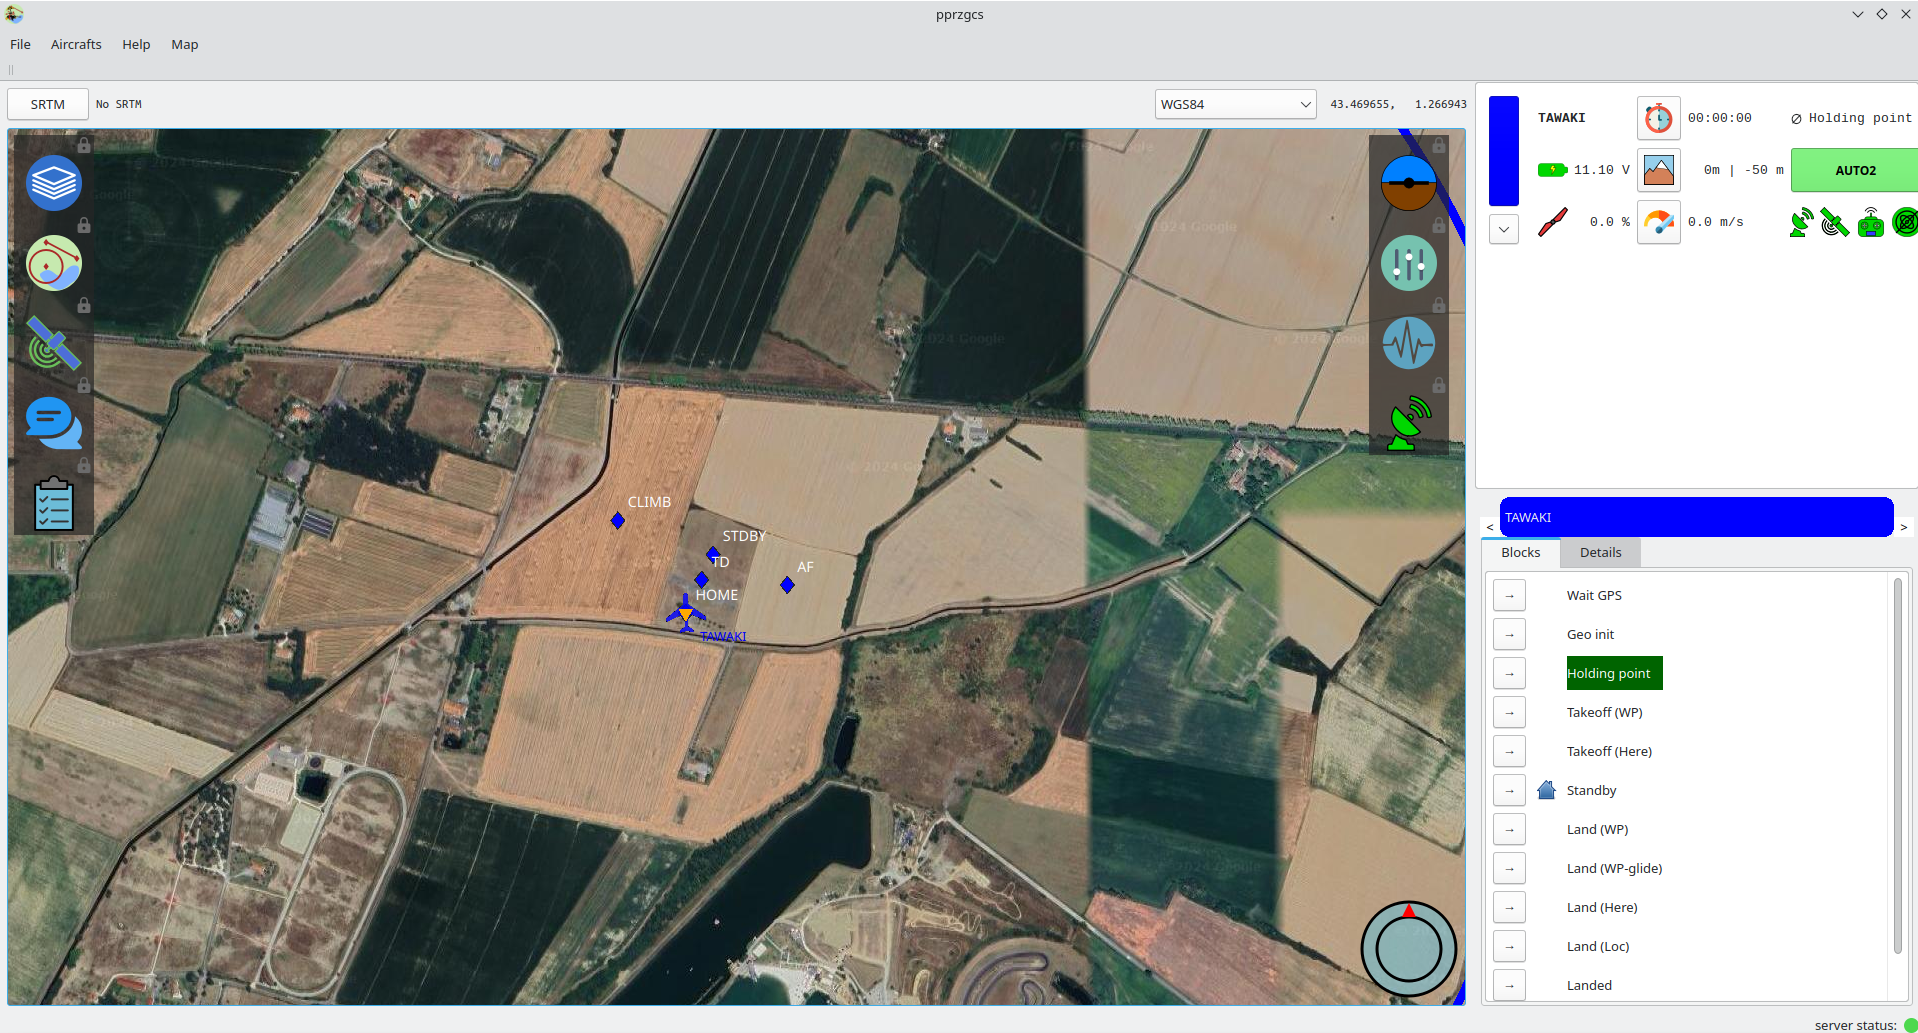
\includegraphics[trim=0cm 0cm 0cm 0cm,clip,width=0.8\columnwidth]{figures/GCS.png}}
    \caption{Interface graphique de la station de contrôle au sol.}
    \label{fig:GCS}
\end{figure}

\nomenclature[]{\(GCS\)}{Station de contrôle au sol \textit{Ground Control Station}}

Une autre partie du segment sol est le code serveur qui gère les messages échanger entre les différentes applications. Le code est en Ocaml.

Enfin, un code assure la compilation croisée du logiciel embarqué qui doit être téléversé sur le drone, basée sur des Makefile et du code Ocaml. Le logiciel embarqué est décrit par la suite.

 \subsection{Le logiciel embarqué}
 Le logiciel embarqué est un code écrit en C, intégré dans un système d'exploitation temps réel "Chibios". Il est téléversé sur le microcontrôleur au travers d'une sonde de programmation ou de la prise USB présente sur l'autopilote.

 L'ensemble du code est organisé sous la forme de module que l'on change au besoin. Chaque module assurant des fonctionnalités telles que l'estimation d'état, la stabilisation, le guidage, la navigation ou encore la gestion de la charge utile (voir figure \ref{fig:schedulingpaparazzi}). Grâce à un mécanisme de gestion de dépendance, les modules ont la possibilité de charger d'autre module nécessaire à leur fonctionnement. L'ordre de compilation et d'édition des liens sera géré par le logiciel de compilation.


 \begin{figure}[ht!]
    \centerline{
    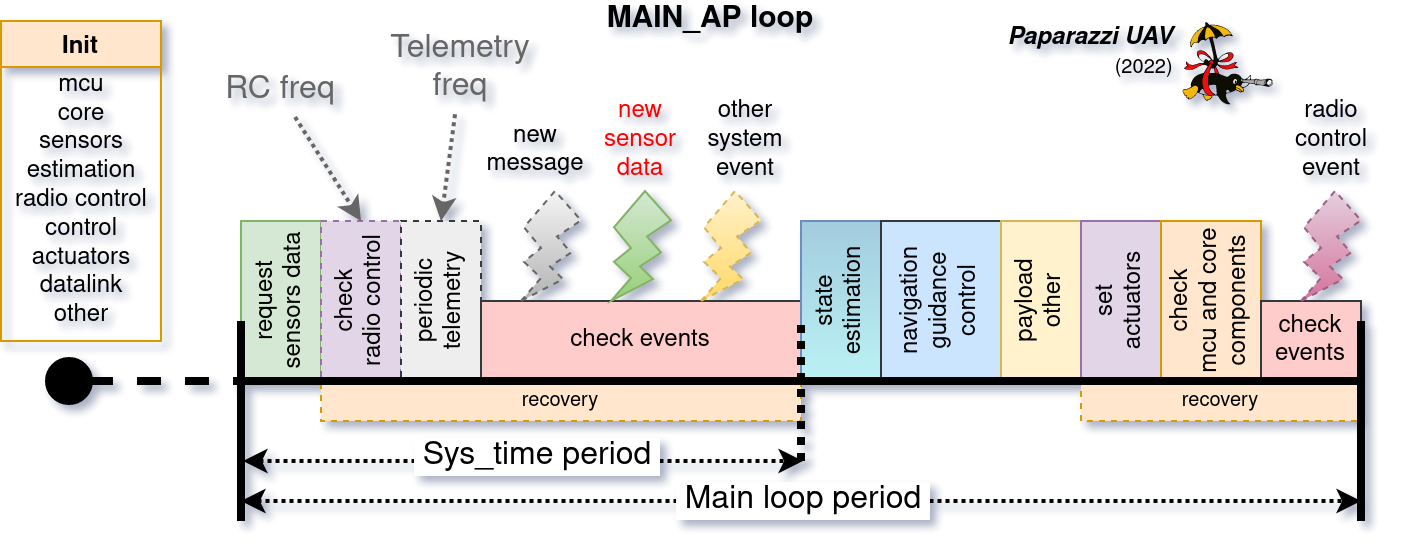
\includegraphics[trim=0cm 0cm 0cm 0cm,clip,width=0.7\columnwidth]{figures/PPRZ_Main_ap_loop.png}}
    \caption{Schéma de l'ordre d'exécution des codes embarqués \cite{RTDpaparazzi2022}.}
    \label{fig:schedulingpaparazzi}
\end{figure}

 
\section{AM32}
\label{sec:AM32}
Le logiciel AM32 est conçu pour les microprocesseurs ARM STM32 afin de contrôler un moteur \textit{brushless}, couramment utiliser pour les drones. Le logiciel est conçu pour être sûr et rapide, avec des démarrages rapides et sans à-coups et une accélération linéaire. Il est destiné à être utilisé avec plusieurs types de véhicules et de contrôleur de vol. 

L'intérêt de ce logiciel est qu'il est ouvert, ainsi il est possible de contribuer en proposant des évolutions. Ce que nous avons fait implémentant l'approche de \cite{franchi2017}, avec un algorithme de biais et de gain adaptatif (ABAG) (voir \ref{fig:ABAG_algo}).

\begin{figure}[ht!]
    \centerline{
    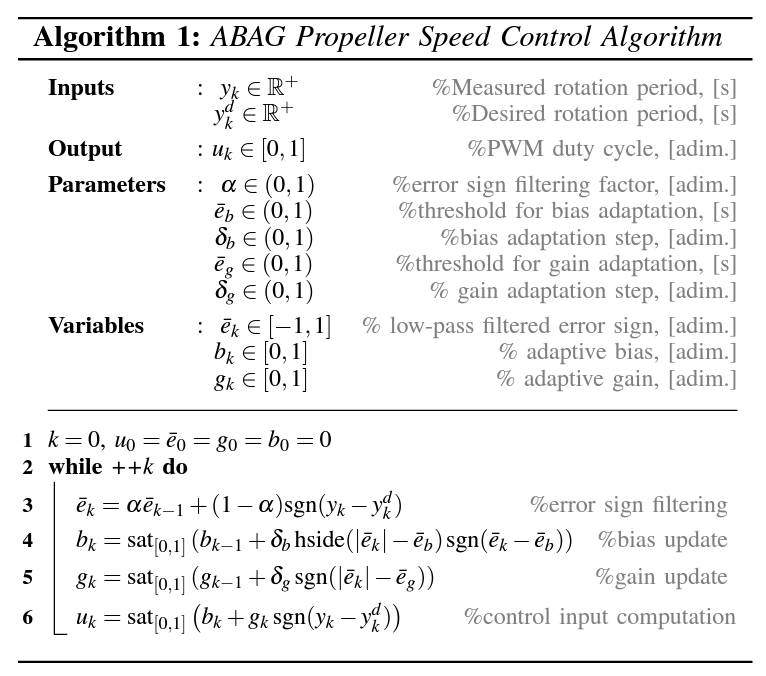
\includegraphics[trim=0cm 0cm 0cm 0cm,clip,width=0.6\columnwidth]{figures/ABAG_algo.png}}
    \caption{Algorithme de biais et de gain adaptatif (ABAG) \cite{franchi2017}.}
    \label{fig:ABAG_algo}
\end{figure}
L'algorithme ABAG est adaptatif et robuste en ce sens qu'il ne nécessite pas la connaissance des paramètres mécaniques ou électriques du groupe moteur et hélice et qu'il n'est pas nécessaire de procéder à une identification, ni de connaître l'entrée nominale. De plus, l'algorithme ABAG ne nécessite que très peu de ressource de calcul, ce qui en fait un atout important pour un système embarqué.

 }